%% latex_template.tex
%%
%% The following file is a skeleton file that demonstrates how to implement the IEEEtran.cls class 
%% file in LaTeX. This file is intended as a template for academic and technical writing in 
%% the LaTeX environment.
%%
%% This file is heavily adapted from Michael Shell's bare_adv.tex file made available at 
%% http://www.ieee.org/conferences_events/conferences/publishing/templates.html
%%
%% You will need to rename this file with your information in the following format:
%% latex_185_last name_ first initial.tex
%% ---------------------------------------------------------------------------------------------------

% \documentclass{} precedes the preamble and is typically the first command in any .tex document. Every .tex document should include this command as it defines what kind of document you intend on creating. Modifiers in square brackets [] can be added in between the text ''documentclass'' and the curly brackets {} to modify font size, templates, etc. 

\documentclass[12pt,journal,compsoc]{IEEEtran}

%-----PACKAGES-------------------------------------------------------------------------------------

% Packages include extra commands that allow for additional formatting, ranging from Graphics, Math, to Alignment. The command to include packages will always look similar to \usepackage{} where the package name is within the curly brackets {}. Packages are defined in the preamble, i.e., between the \documentclass{} and \begin{document} commands.

% The following link takes you to a list of additional packages that may not be listed here. http://en.wikibooks.org/wiki/LaTeX/Package_Reference

% TO INCLUDE PACKAGES: 
% - Open the file ''latex_sample_packages.tex'' from the .zip folder.
% - From this file, COPY the code for the package you want to include and PASTE into your own .tex file.
% - Uncomment the package you want to include and load, i.e., remove the ''%'' in front of the \usepackage{package_name}.
 

% Copy package text here:

\usepackage{graphicx}
\usepackage{url}
\usepackage{tikz}
\usepackage{pgfplots}
\pgfplotsset{compat=1.18}
% This is an example of how a \usepackage{} command should be included. You will need to include more packages to complete this assignment.




%----- The DOCUMENT Environment-------------------------------------------------------------------

% The \begin{document} and \end{document} commands establish the environment for the text of the document. The \begin{} and \end{} commands are used repeatedly in LaTeX to show where an environment begins and ends. The \end{document} command will be the last line of this .tex file.

\begin{document}

% The following commands are self explanatory. Insert your title, author and date into each command's curly bracket. You can include the abstract, paper header and paper footer information in this section then conclude the section with the command \maketitle (shown as the last line at the end of this section).

\title{A Beginner's Guide to LaTeX: Using IEEEtran.cls for Academic Writing}
\author{Author~Name}
% The double backslash \\ is used here to enter a ''Carriage Return'', or a line break. Note that the tilde ~ in between my name used as a ''Nonbreaking Space''. LaTeX will not break a structure at a ~ so this keeps an author's name from being broken across two lines. Also note that I included my name as an example so make sure to only insert your name in this command.

\date{}		% leaving the brackets empty omits the date
% To input the current date, you can type: \date{\today}

% The paper headers
\markboth{\LaTeX\ IEEE Template Tutorial}%
{Author: Course Name}
% The only time the second header will appear is for the odd numbered pages
% after the title page when using the twoside option.
% 
% *** Note that you probably will NOT want to include the author's ***
% *** name in the headers of peer review papers.                   ***
% You can use \ifCLASSOPTIONpeerreview for conditional compilation here if
% you desire.

% The publisher's ID mark at the bottom of the page is less important with
% Computer Society journal papers as those publications place the marks
% outside of the main text columns and, therefore, unlike regular IEEE
% journals, the available text space is not reduced by their presence.
% If you want to put a publisher's ID mark on the page you can do it like
% this:
\IEEEpubid{0000--0000/00\$00.00~\copyright~2007 IEEE}
% or like this to get the Computer Society new two part style.
%\IEEEpubid{\makebox[\columnwidth]{\hfill 0000--0000/00/\$00.00~\copyright~2007 IEEE}%
%\hspace{\columnsep}\makebox[\columnwidth]{Published by the IEEE Computer Society\hfill}}
% Remember, if you use this you must call \IEEEpubidadjcol in the second
% column for its text to clear the IEEEpubid mark (Computer Society jorunal
% papers don't need this extra clearance.)


% use for special paper notices
%\IEEEspecialpapernotice{(Invited Paper)}

% for Computer Society papers, we must declare the abstract and index terms
% PRIOR to the title within the \IEEEcompsoctitleabstractindextext IEEEtran
% command as these need to go into the title area created by \maketitle.
\IEEEcompsoctitleabstractindextext{%
\begin{abstract}
This tutorial provides a comprehensive introduction to \LaTeX\ document preparation for novice users, with a focus on academic and technical writing. Using the IEEEtran.cls document class, readers will learn essential \LaTeX\ concepts including document structure, text formatting, mathematical expressions, figures, tables, citations, and bibliography management. The guide covers practical examples and best practices for creating professional IEEE-style documents suitable for academic papers, theses, and technical reports.
\end{abstract}
% IEEEtran.cls defaults to using nonbold math in the Abstract.
% This preserves the distinction between vectors and scalars. However,
% if the journal you are submitting to favors bold math in the abstract,
% then you can use LaTeX's standard command \boldmath at the very start
% of the abstract to achieve this. Many IEEE journals frown on math
% in the abstract anyway. In particular, the Computer Society does
% not want either math or citations to appear in the abstract.

% Note that keywords are not normally used for peerreview papers.
\begin{IEEEkeywords}
\LaTeX, IEEEtran, academic writing, document preparation, typesetting.
\end{IEEEkeywords}}

\maketitle

%----- The SECTION Environment -------------------------------------------------------------------

% To create a section, simply type the command \section{} with the name of your section name inserted into the curly brackets {}. The section's body text follows underneath the \section{} command. 

\section{Introduction}

\IEEEPARstart{W}{elcome} to this beginner's guide to \LaTeX, the popular document preparation system used extensively in academic and technical writing. \LaTeX\ is a content-focused system; it emphasizes content over design, thus allowing users to produce professionally formatted documents with uniformity and high-quality typesetting.

This tutorial is aimed at students and professionals with no prior experience of \LaTeX\ looking to produce their own academic papers, theses, and technical reports. This tutorial will use the IEEEtran.cls document class, which is based upon the IEEE publishing guidelines (IEEE) and also commonly used in the majority of academic institutions. Using practical examples and step-by-step guidance, you will be able to develop the necessary skills to work with the main components of creating a \LaTeX\ document.


%----- Additional Features -----------------------------------------------------------------------

\section{Additional Features}

\subsection{Figures}
Figures are essential for technical documents and \LaTeX\ provides excellent support for including and formatting images. The \texttt{figure} environment allows you to include graphics while maintaining proper document flow.

The \texttt{figure} environment is created using \verb|\begin{figure}| and \verb|\end{figure}| commands. This environment creates a floating object that \LaTeX\ can position automatically to maintain good page layout. Within the figure environment, you typically include:

\begin{itemize}
\item \verb|\centering|: Centers the image horizontally
\item \verb|\includegraphics{filename}|: Inserts the image file
\item \verb|\caption{text}|: Adds a caption below the figure
\item \verb|\label{marker}|: Creates a reference label for cross-referencing
\end{itemize}

% FIGURES:

% Note the FIGURE Environment created by the \begin{figure} and \end{figure} commands.

% Uncomment and add your own image file when using this template:
% \begin{figure}[h] 	% There are several different modifiers that can be used in [].
% \centering
% \includegraphics[width=1.5in]{your-image.pdf}
% \caption{Example Figure}
% \label{fig_example}
% \end{figure}

Note that the \verb|\caption| command should come before \verb|\label|, and the \verb|\label| must come after \verb|\caption| for proper cross-referencing. The image file (in this case, \texttt{your-image.pdf}) must be in the same directory as your \texttt{.tex} file, or you must specify the full path to the image.

The \texttt{graphicx} package provides the \verb|\includegraphics| command, which supports various image formats including PDF, PNG, JPG, and EPS. Key parameters include:
\begin{itemize}
\item \texttt{[width=]}: Set absolute width
\item \texttt{[height=]}: Set absolute height
\item \texttt{[scale=]}: Scale relative to original size
\item \texttt{[angle=]}: Rotate the image
\end{itemize}

The figure placement options in square brackets control where \LaTeX\ positions the figure:
\begin{itemize}
\item \texttt{h}: Here (approximately)
\item \texttt{t}: Top of page
\item \texttt{b}: Bottom of page
\item \texttt{p}: Separate page for floats
\item \texttt{!}: Override restrictions
\end{itemize}

% You will need to use appropriate file types for figures and will also need to include that image file in the same folder as your .tex file. 

\subsubsection{Creating Plots with \LaTeX}
\LaTeX\ can also create plots directly using the \texttt{pgfplots} package. This is particularly useful for scientific data visualization. The following example demonstrates creating a titration curve plot from experimental data:

\begin{figure}[h]
\centering
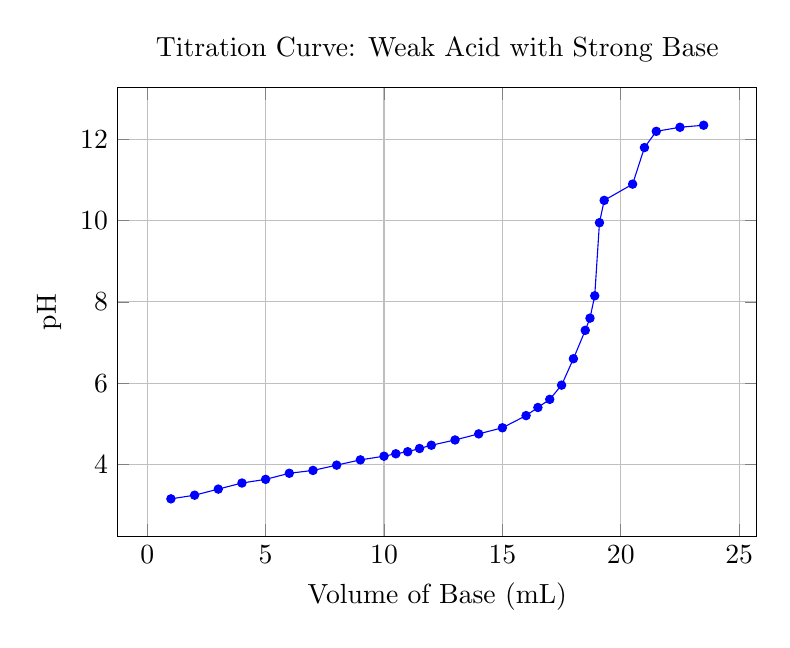
\begin{tikzpicture}
\begin{axis}[
    width=0.8\columnwidth,
    height=0.6\columnwidth,
    xlabel={Volume of Base (mL)},
    ylabel={pH},
    grid=major,
    legend pos=south east,
    title={Titration Curve: Weak Acid with Strong Base}
]
\addplot[color=blue,mark=*,mark size=1.5pt] coordinates {
    (1.00,3.15) (2.00,3.24) (3.00,3.39) (4.00,3.54) (5.00,3.63)
    (6.00,3.78) (7.00,3.85) (8.00,3.98) (9.00,4.11) (10.00,4.20)
    (10.50,4.26) (11.00,4.31) (11.50,4.39) (12.00,4.47) (13.00,4.60)
    (14.00,4.75) (15.00,4.90) (16.00,5.20) (16.50,5.40) (17.00,5.60)
    (17.50,5.95) (18.00,6.60) (18.50,7.30) (18.70,7.60) (18.90,8.15)
    (19.10,9.95) (19.30,10.50) (20.50,10.90) (21.00,11.80) (21.50,12.20)
    (22.50,12.30) (23.50,12.35)
};
\end{axis}
\end{tikzpicture}
\caption{Titration curve showing pH versus volume of NaOH added. The sharp rise in pH indicates the equivalence point, which occurs around 19 mL. This plot was created using the \texttt{pgfplots} package in \LaTeX\ from experimental titration data.}
\label{fig:titration}
\end{figure}

To create this plot, the \texttt{pgfplots} package is loaded in the preamble with \verb|\usepackage{pgfplots}|. The plot is created within a \texttt{tikzpicture} environment using an \texttt{axis} environment. Data points are specified using the \verb|\addplot| command with \verb|coordinates|, and the plot is customized with axis labels, grid, and title options.

%-------------------------------------------------------------------------------------------------
\subsection{Label, Cite, and Ref Commands}
Cross-referencing is one of \LaTeX's most powerful features, allowing you to automatically number and reference sections, figures, tables, and equations.

\subsubsection{Labels and References}
The \verb|\label{marker}| command assigns a reference marker to the current location. You can then reference this marker using \verb|\ref{marker}|, which will display the automatically generated number.

\begin{verbatim} \label{fig_example} \end{verbatim} as it appears in the figure environment\\
% \begin{verbatim} \ref{fig_example} \end{verbatim} appears like: \ref{fig_example} (commented out)\\

Labels work with:
\begin{itemize}
\item \textbf{Sections:} \texttt{\textbackslash section\{Title\}} \\
  \texttt{\textbackslash label\{sec:intro\}}
\item \textbf{Subsections:} \texttt{\textbackslash subsection\{Title\}} \\
  \texttt{\textbackslash label\{subsec:methods\}}
\item \textbf{Figures:} \texttt{\textbackslash caption\{Caption\}} \\
  \texttt{\textbackslash label\{fig:results\}}
\item \textbf{Tables:} \texttt{\textbackslash caption\{Caption\}} \\
  \texttt{\textbackslash label\{tab:data\}}
\item \textbf{Equations:} \texttt{\textbackslash label\{eq:formula\}}
\end{itemize}

\subsubsection{Citations and Bibliography}
The \verb|\cite{key}| command creates citations that link to your bibliography entries. The key corresponds to the bibliography entry identifier.

\begin{verbatim} \cite{IEEEhowto:kopka} \end{verbatim} appears like: \cite{IEEEhowto:kopka}\\

Multiple citations can be combined: \verb|\cite{key1,key2}| produces \cite{IEEEhowto:kopka}.

% IMPORTANT NOTE: In order to assign the correct reference number to each label, you may have to compile your code twice. 

%-------------------------------------------------------------------------------------------------
\subsection{Tables}
Tables organize data in rows and columns and are created using the \texttt{table} environment with the \texttt{tabular} environment inside.

% An example of a floating table. Note that, for IEEE style tables, the
% \caption command should come BEFORE the table. Table text will default to
% \footnotesize as IEEE normally uses this smaller font for tables.
% The \label must come after \caption as always.
%
\begin{table}[h]
%% increase table row spacing, adjust to taste
\renewcommand{\arraystretch}{1.3}
% if using array.sty, it might be a good idea to tweak the value of
%\extrarowheight as needed to properly center the text within the cells
\caption{An Example of a Table}
\label{table_example}
\centering
%% Some packages, such as MDW tools, offer better commands for making tables
%% than the plain LaTeX2e tabular which is used here.
\begin{tabular}{|c||c|}
\hline
One & Two\\
\hline
Three & Four\\
\hline
\end{tabular}
\end{table}

The \texttt{tabular} environment uses column specifications:
\begin{itemize}
\item \texttt{l}: Left-aligned column
\item \texttt{c}: Centered column
\item \texttt{r}: Right-aligned column
\item \texttt{p\{width\}}: Paragraph column with specified width
\item \texttt{|}: Vertical line between columns
\end{itemize}

Use \verb|&| to separate cells and \verb|\\| to end rows. The \verb|\hline| command adds horizontal lines.

\subsection{Mathematical Expressions}
\LaTeX\ excels at typesetting mathematical expressions using \TeX's built-in math capabilities. Math can be displayed inline using single dollar signs (\verb|$...$|) or as separate equations using double dollar signs (\verb|$$...$$|) or the \texttt{equation} environment.

Inline math: $E = mc^2$ shows how formulas integrate with text.

Display equations use the \texttt{equation} environment:
\begin{equation}
\sum_{i=1}^{n} x_i = \int_{0}^{1} f(x) \, dx
\label{eq:sum}
\end{equation}

Common mathematical symbols and commands include:
\begin{itemize}
\item Superscripts: \verb|x^2| produces $x^2$
\item Subscripts: \verb|x_i| produces $x_i$
\item Fractions: \verb|\frac{a}{b}| produces $\frac{a}{b}$
\item Greek letters: \verb|\alpha, \beta, \gamma| produces $\alpha, \beta, \gamma$
\item Operators: \verb|\sum, \int, \lim| produce $\sum, \int, \lim$
\end{itemize}

\subsection{Document Structure and Formatting}
\LaTeX\ documents have a hierarchical structure that helps organize content logically.

\subsubsection{Sections and Headings}
\begin{itemize}
\item \verb|\section{Title}|: Major section divisions
\item \verb|\subsection{Title}|: Subdivisions within sections
\item \verb|\subsubsection{Title}|: Further subdivisions
\item \verb|\paragraph{Title}|: Paragraph-level headings
\end{itemize}

\subsubsection{Text Formatting}
Basic text formatting commands include:
\begin{itemize}
\item \verb|\emph{text}|: Emphasis (italics)
\item \verb|\textbf{text}|: Bold text
\item \verb|\texttt{text}|: Monospace font
\item \verb|\textsc{text}|: Small caps
\end{itemize}

\subsubsection{Special Characters}
Some characters have special meanings in \LaTeX\ and must be escaped:
\begin{itemize}
\item \verb|\&| for \& (ampersand)
\item \verb|\%| for \% (percent sign)
\item \verb|\$| for \$ (dollar sign)
\item \verb|\#| for \# (hash symbol)
\item \verb|\_| for \_ (underscore)
\item \verb|\{| and \verb|\}| for \{ and \}
\end{itemize}

\subsection{Packages and Document Classes}
The \verb|\documentclass| command at the beginning of your document defines the overall formatting style. IEEEtran.cls is specifically designed for IEEE publications and provides:
\begin{itemize}
\item Two-column layout
\item Proper heading styles
\item Bibliography formatting
\item Figure and table placement rules
\end{itemize}

Packages extend \LaTeX's capabilities. Essential packages include:
\begin{itemize}
\item \texttt{graphicx}: Image inclusion
\item \texttt{amsmath}: Advanced mathematical typesetting
\item \texttt{geometry}: Page layout control
\item \texttt{hyperref}: PDF hyperlinks and bookmarks
\end{itemize}

Packages are loaded in the preamble using \verb|\usepackage[options]{package-name}|.


\section{Conclusion}

You have now been exposed to the key principles and practical aspects of working with \LaTeX\ to create academic documents to a professional standard using the IEEEtran.cls document class. In addition to understanding how to structure your documents, how to format your text, how to include mathematical expressions into your document, how to insert and manage figures and tables, and how to add citations and references to your bibliography, you have also learned how to make full use of \LaTeX's advantages in producing academic documents, including:

\begin{itemize}
\item Superior typesetting quality;
\item Automatic reference cross-referencing capabilities;
\item Consistency in producing large documents;
\end{itemize}

While there may be a time commitment involved with learning \LaTeX, the benefits of being able to produce manuscript-ready documents far outweigh the costs.

As you progress with your \LaTeX\ journey, I would recommend investigating other package options that could help with more specific requirements, such as:

\begin{itemize}
\item Algorithm document formatting,
\item Chemical structures, and
\item Advanced mathematics document formatting.
\end{itemize}

There are several online resources available to support your continued \LaTeX\ development, such as:

\begin{itemize}
\item \LaTeX\ Wikibook,
\item TeX Stack Exchange, and
\item Overleaf Documentation.
\end{itemize}

Practice is key when developing your \LaTeX\ skills. As you gain confidence with the \LaTeX\ system, begin by producing simple documents and then build up to incorporating more complex document features.

The IEEEtran.cls document class that has been employed throughout this tutorial offers a solid base from which to proceed with your academic and technical writing.

%----- APPENDICES --------------------------------------------------------------------------------
\appendices
\section{Common \LaTeX\ Commands Reference}
This appendix provides a quick reference for frequently used \LaTeX\ commands.

\subsection{Text Formatting Commands}
Common text formatting commands include:
\begin{itemize}
\item \texttt{\textbackslash emph\{text\}} produces \emph{emphasized text} (italic emphasis)
\item \texttt{\textbackslash textbf\{text\}} produces \textbf{bold text} (bold formatting)
\item \texttt{\textbackslash texttt\{text\}} produces \texttt{monospace text} (typewriter font)
\item \texttt{\textbackslash textsc\{text\}} produces \textsc{small caps text} (small capital letters)
\item \texttt{\textbackslash underline\{text\}} produces \underline{underlined text} (underlined text)
\end{itemize}

\subsection{Mathematical Symbols}
Common mathematical symbols and their commands:
\begin{itemize}
\item Greek letters: $\alpha, \beta, \gamma, \delta, \epsilon, \theta, \lambda, \mu, \pi, \sigma, \phi, \omega$
\item Operators: $\pm, \times, \div, \cdot, \circ, \oplus, \otimes$
\item Relations: $\leq, \geq, \neq, \approx, \equiv, \propto, \sim$
\item Arrows: $\leftarrow, \rightarrow, \uparrow, \downarrow, \leftrightarrow$
\item Miscellaneous: $\infty, \partial, \nabla, \int, \sum, \prod, \bigcup, \bigcap$
\end{itemize}

\section{\LaTeX\ Document Compilation}
% you can choose not to have a title for an appendix
% if you want by leaving the argument blank
\subsection{Compilation Process}
To compile a \LaTeX\ document:

\begin{enumerate}
\item Save your \texttt{.tex} file
\item Run \texttt{pdflatex} or \texttt{xelatex} on the file
\item For documents with bibliography, run \texttt{bibtex} then \texttt{pdflatex} twice more
\item Open the resulting \texttt{.pdf} file
\end{enumerate}

\subsection{Troubleshooting Common Errors}
\begin{itemize}
\item \textbf{Missing package}: Install required packages using your \TeX\ distribution's package manager
\item \textbf{Undefined control sequence}: Check for typos in command names
\item \textbf{Missing \texttt{\textbackslash begin\{document\}}} or similar: Ensure all environments are properly opened and closed
\item \textbf{File not found}: Verify image files are in the correct directory
\item \textbf{Reference undefined}: Compile document multiple times for cross-references to resolve
\end{itemize}

\subsection{Recommended Tools and Editors}
\begin{itemize}
\item \textbf{Overleaf}: Web-based \LaTeX\ editor with real-time collaboration
\item \textbf{TeXstudio}: Feature-rich editor with integrated PDF viewer
\item \textbf{VS Code + \LaTeX\ extensions}: Modern editor with \LaTeX\ support
\item \textbf{TeX Live}: Comprehensive \TeX\ distribution for all platforms
\end{itemize}


%----- ACKNOWLEDGEMENT SECTION -------------------------------------------------------------------
% Explain what the asterisk * does in the next line:
\section*{Acknowledgements}

The author would like to thank the course instructor for providing guidance and materials that served as the foundation for this tutorial. Special thanks to the course staff for their support in technical writing and \LaTeX\ usage.

This tutorial draws from Michael Shell's IEEEtran documentation and various online \LaTeX\ resources including the \LaTeX\ Wikibook and TeX Stack Exchange community.

The asterisk (*) after \verb|\section| creates an unnumbered section that doesn't appear in the table of contents, which is appropriate for acknowledgments in academic papers.

The bibliography environment contains all cited references in your document. Each \verb|\bibitem{key}| creates a reference entry that can be cited using \verb|\cite{key}|. The bibliography automatically numbers entries and formats them according to the document style.

% You will need to explain how to include the bibliography section as follows. Explain the environment and how to add new items.
% Including how \ref, \cite and \label should be included here.

\vspace{0.2in}
\begin{thebibliography}{1}

\bibitem{IEEEhowto:kopka}
H.~Kopka and P.~W. Daly, \emph{A Guide to {\LaTeX}}, 3rd~ed.\hskip 1em plus
  0.5em minus 0.4em\relax Harlow, England: Addison-Wesley, 1999.

\bibitem{lamport1994latex}
L.~Lamport, \emph{{\LaTeX}: A Document Preparation System}, 2nd~ed.\hskip 1em plus
  0.5em minus 0.4em\relax Reading, MA: Addison-Wesley, 1994.

\bibitem{goossens1994latex}
M.~Goossens, F.~Mittelbach, and A.~Samarin, \emph{The {\LaTeX} Companion},
  1st~ed.\hskip 1em plus 0.5em minus 0.4em\relax Reading, MA: Addison-Wesley, 1994.

\bibitem{wikibook}
{\LaTeX} community, \emph{{\LaTeX} Wikibook}, accessed October 2023.
  Available: \url{https://en.wikibooks.org/wiki/LaTeX}

\bibitem{shell2007ieee}
M.~Shell, \emph{IEEEtran {\LaTeX} Class}, accessed October 2023.
  Available: \url{https://www.ieee.org/conferences_events/conferences/publishing/templates.html}

\end{thebibliography}

%----- Optional: BIOGRAPHY Section ---------------------------------------------------------------

% If you have an EPS/PDF photo (graphicx package needed) extra braces are
% needed around the contents of the optional argument to biography to prevent
% the LaTeX parser from getting confused when it sees the complicated
% \includegraphics command within an optional argument. (You could create
% your own custom macro containing the \includegraphics command to make things
% simpler here.)
% Uncomment and modify the following section if you want to include a biography:
%
% \begin{IEEEbiography}[{\raisebox{-0.3\height}{\includegraphics[width=1in,height=1.25in,clip,keepaspectratio]{profile.jpg}}}]{Author Name}
% Author Name is currently pursuing their undergraduate degree in Computer
% Engineering. They have developed a
% strong foundation in technical writing, particularly using \LaTeX, during their coursework in technical writing. This tutorial represents their work
% in mastering \LaTeX\ document preparation.
% \end{IEEEbiography}


% insert where needed to balance the two columns on the last page with
% biographies
%\newpage

% You can push biographies down or up by placing
% a \vfill before or after them. The appropriate
% use of \vfill depends on what kind of text is
% on the last page and whether or not the columns
% are being equalized.

%\vfill

% Can be used to pull up biographies so that the bottom of the last one
% is flush with the other column.
%\enlargethispage{-5in}

\end{document}
